\chapter{Background}\label{chap:bkg}

%TODO more math and explain it

\section{Cell-free systems}
\gls{cfps} systems have existed since the early 1960's as a way to express proteins that are otherwise difficult to express in a living cell~\cite{nirenberg1961dependence}.
These early \gls{cfps} systems were quite crude and had low protein yields, limiting their utility.
More recently, work involving the removal of certain genes~\cite{calhoun2006total} and the improved stability of cofactor regeneration pathways~\cite{jewett2008integrated} has allowed for improved yield of \gls{cfps} systems.
%stabilized amino acid synthesis leading to 
%Another crucial development was the ability to ensure cofactor regeneration pathways were maintained in the \gls{cfps} system}.
%These recent improvements in \gls{cfps} systems have led to a multitude of applications for cell-free technologies~\cite{}.

When discussing \gls{cfps} systems, it is important to distinguish between the multiple types of cell-free systems.
One type of cell-free system is created by combining individual purified proteins involved in transcription and translation.
The most widely utilized of these reconstituted cell-free systems is the PURE system~\cite{shimizu2001cell}.
The benefit of these systems is that the system is completely known and controlled.
Since the only things in the system are the proteins that have been deliberately aded, users of the systems can be assured that there are no undesirable elements such as nucleases or proteases present.
However, these systems have relatively high costs due to the time and effort required to isolate and purify each of the requisite proteins.

The type of \gls{cfps} system we use in this dissertation is an extract-based system created using a crude cell extract.
Creating an extract-based \gls{cfps} system involves growing cells and then lysing them to create a cell extract.
This extract is then used as the basis of the \gls{cfps} system with the assumption that all the important transcription/translation machinery remains intact in the cell extract.
Growing up large quantities of cells is relatively cheap, so these types of systems have the potential to scale more effectively than reconstituted cell-free systems. 
The downside to this method of creating \gls{cfps} systems is that the exact composition of these cell extracts is unknown and could potentially vary between batches of \gls{cfps} systems.
This motivates our work to provide an accurate model of these crude \gls{cfps} systems.

\section{Flux Balance Analysis}
Flux Balance Analysis (\gls{fba}) is one of the most common metabolic modeling tools.
\gls{fba} relies on a mathematical representation of all of the metabolic reactions occurring in an organism.
These reactions are represented using a matrix $S$, a $M x N$ matrix, where each row represents a separate reaction and each column is a different metabolite.
The entries in this matrix are the stoichiometric coefficient for each metabolite in a given reaction.
Metabolites that are consumed in a reaction are represented using negative numbers.
Flux through each of these reactions can be represented by a vector $v$, which is a 1-dimension vector with a length equal to the number of the reactions.
A crucial assumption in \gls{fba} is that the system is at steady state, so the overall flux through all of the reactions is not changing.
We can represent this by writing the following:
\begin{equation}
S * v = 0 \\
\end{equation}
where $S$ is the known stoichiometric matrix and $v$ is the unknown flux vector.
The goal of \gls{fba} is to solve for $v$.

This system is underspecified---we typically have more reactions than metabolites ($N >> M$)---so there is no unique solution to this equation.
We deal with this issue by specifying additional constraints on our flux vector $v$.
We can specify constraints on different reactions in order to limit the amount of flux proceeding through a given reaction.
For instance, we represent reaction as irreversible by setting the lower bound on that reaction to be 0.
This specifies that it can only proceed in one direction and ensures that the model reflects the underlying biology.
We use \gls{lp} to solve this constrained, underspecified system. 

In order to find an optimal solution to this problem, we first need to specify an objective function.
This objective function determines the which fluxes are most phenotypically relevant.
When choosing an objective function, we can either choose a specific reaction to optimize the flux through or create a pseudo-reaction that contains a combination of important metabolites.
A common choice of objective function is the Biomass Objective Function, which incorporates many essential metabolites necessary for cell growth~\cite{feist2010biomass}.
While some of our models use the Biomass Objective Function, we also use the production of a specific product as our objective function.
In the general case, we can represent our objective function as $Z$.
We can specify which reactions are part of the objective function using the vector $c$.

Now we can reformulate our problem to be a \gls{lp} problem of the form:
\begin{equation}
\centering
\begin{split}
\text{max } Z &= c^Tv \\
&\text{s.t. } S * v = 0 \\
&\text{and } -1000 < v_0 < 1000 \\
&\text{and } 0 < v_1 < 1000 \\
...
\end{split}
\end{equation}
where $v_i$ is the flux through reaction $i$.
We can then use a \gls{lp} solver to find the optimal solution to this problem.
%It may be useful to imagine the potential space of all \gls{fba} solutions that can satisfy the constraints as a hypercube.
%Then, the linear programming solver finds an optimum at one corner of the hypercube based on the objective function.

The use of \gls{fba} involves this key steady state assumption---i.e. the system is stable.
\gls{cfps} systems are dynamic systems and do not have a period where intake and output are equal until the system is no longer producing protein.
However, we can consider the period of maximal production of a \gls{cfps} system to be its steady state.
Thus, we can use \gls{fba} to analyze this pseudo-steady state, which is the period that we are interested in.

%A typical \gls{fba} model includes thousands of reactions; this is extremely high dimensional data.
%In order to extract insights from the data, we need to use dimensionality reduction techniques.

\section{Autoencoders}
Autoencoders are a dimensionality reduction technique with a very simple idea: given a dataset, try to reconstruct that dataset by passing it through a lower dimensional subspace.
This is performed by training an encoder network that learns how to map from the original dataset to the lower dimensional data and a decoder network that can map from the low dimensional subspace back to the subspace of the original data.
The original idea behind autoencoders was that this lower dimensional representation of the data functioned as a compressed version of the data.
Instead of hand designing compression/decompression algorithms, these functions can be learned to be application specific.
These autoencoders are often worse than hand-designed compression algorithms and have difficulty competing with classic algorithms on problems such as image compression~\cite{theis2017lossy}.
However, the lower dimensional compressed representation can be used as a dimensionality reduction technique to uncover non-obvious relationships within the original data.
This is similar to the idea behind \gls{pca}, though \gls{pca} projects the data into a subspace in a linear manner, while autoencoders are able to learn non-linear transformation.

\begin{figure}[t!]
\begin{center}
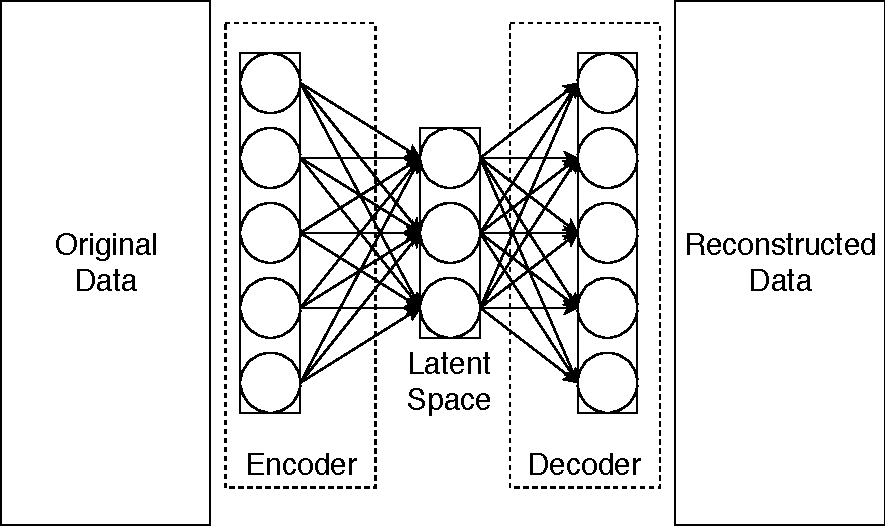
\includegraphics{figs/Autoencoder.pdf}
\caption{Example of a single layer autoencoder.
In this case, both the encoder and the decoder are a single layer neural network.
These layers can be stacked to create even more complex dimensionality reductions.}
\end{center}
\label{fig:ae}
\end{figure}

The implementation of autoencoders usually uses neural network layers to learn the encoding and decoding functions.
Figure \ref{fig:ae} demonstrates an example structure of a very simple autoencoder.
There are a number of different types of autoencoders that are extensions of this basic idea.
One example is a sparse autoencoder.
In order to force the autoencoder to learn a more general dimensionality reduction, we can add a sparsity constraint to limit the number of activations among the network layers.
This forces the autoencoder to learn a representation with sparse network weights.
Another type of autoencoder is a denoising autoencoder.
This type of autoencoder involves taking a noisy representation and mapping it back to a clean representation of the data.
This can either be trained on noisy data or it can be given the original representation, corrupt it, and then try to learn the original representation from the corrupted data.

Sometimes we want to do more than just learn arbitrary encoding and decoding functions.
For instance, we might want to impose constraints on the encoded representation, also known as the latent space.
\glspl{vae} are a class of autoencoder that does exactly this.
\glspl{vae} constrain the encoded representation to be a probability distribution.
So, instead of learning functions that encode/decode the data, the \gls{vae} actually learns the parameters of the encoded probability distribution.
Specifically, the encoder learns to map samples to a mean and standard deviation, which is our latent space.
Then, when decoding the sample, we can sample randomly using the encoded mean and standard deviation as parameters for our probability distribution.

We measure loss in this scheme through a combination of two loss terms.
First, we still care about how well we are able to reconstruct our original data.
So, we can have a reconstruction loss term which measures how well the reconstructed data maps to the original data.
Our second loss term constrains the latent space to ensure that it is well formed and provides a regularization term against overfitting.
We use \gls{kl} divergence, a common way of measuring difference between probability distributions.
We can calculate the the \gls{kl} divergence between our latent space and our prior distribution, which in most cases is a normal distribution.
With the combination of those two loss terms, we can then train the \gls{vae} as we would any other neural network---by using gradient descent to minimize the loss function.

We denote $x_i \in X$ as our data and $z$ as our latent representation.
Our encoder network can be represented by the function $p$ which has parameters $\theta$.
Similarly, our decoder can be represented as a posterior distribution $q$ that is parameterized by $\phi$.
Then the loss function of a \gls{vae} can therefore be written out as follows:

\begin{equation}\label{eqn:vae-loss}
\mathcal{L}(\theta, \phi) = - E[\log p_{\theta}(x_i | z)] + KL(q_{\phi}(z | x_i) || p(z)) \\
\end{equation}

%TODO: add here